\documentclass{article}

\PassOptionsToPackage{numbers,compress}{natbib}
\usepackage[nonanonymous]{neurips_2026}

\usepackage[utf8]{inputenc}
\usepackage[T1]{fontenc}
\usepackage{hyperref}
\usepackage{url}
\usepackage{xurl}
\usepackage{booktabs}
\usepackage{amsfonts}
\usepackage{amsmath}
\usepackage{amssymb}
\usepackage{nicefrac}
\usepackage{microtype}
\usepackage{xcolor}
\usepackage{graphicx}

\setlength{\emergencystretch}{3em}
\Urlmuskip=0mu plus 2mu\relax
\raggedbottom

\makeatletter
\renewcommand{\section}{%
  \@startsection{section}{1}{\z@}%
                {-2.2ex \@plus -0.5ex \@minus -0.2ex}%
                { 1.5ex \@plus  0.3ex \@minus  0.2ex}%
                {\large\bf\raggedright}%
}
\renewcommand{\subsection}{%
  \@startsection{subsection}{2}{\z@}%
                {-2.0ex \@plus -0.5ex \@minus -0.2ex}%
                { 0.8ex \@plus  0.2ex}%
                {\normalsize\bf\raggedright}%
}
\renewcommand{\@maketitle}{%
  \vbox{%
    \hsize\textwidth
    \linewidth\hsize
    \vskip 0.1in
    \@toptitlebar
    \centering
    {\fontsize{13.5}{15.5}\selectfont\bfseries \@title\par}
    \@bottomtitlebar
    \if@anonymous
      \begin{tabular}[t]{c}\bf\rule{\z@}{24\p@}
        Anonymous Author(s) \\
        Affiliation \\
        Address \\
        \texttt{email} \\
      \end{tabular}%
    \else
      \def\And{%
        \end{tabular}\hfil\linebreak[0]\hfil%
        \begin{tabular}[t]{c}\bf\rule{\z@}{24\p@}\ignorespaces%
      }
      \def\AND{%
        \end{tabular}\hfil\linebreak[4]\hfil%
        \begin{tabular}[t]{c}\bf\rule{\z@}{24\p@}\ignorespaces%
      }
      \begin{tabular}[t]{c}\bf\rule{\z@}{24\p@}\@author\end{tabular}%
    \fi
    \vskip 0.3in \@minus 0.1in
  }%
}
\renewcommand{\@notice}{}
\makeatother

\title{CogniSync: Local-First Persistent Memory for MCP-Based Agents}
\author{%
  Saurab Mishra \\
  Indian Institute of Science Education and Research (IISER), Thiruvananthapuram, India \\
  \texttt{saurab23@iisertvm.ac.in}
  \And
  Shubham Mishra \\
  Capgemini, India \\
  \texttt{shubhammishra1204@gmail.com}
}

\begin{document}

\maketitle

\begin{abstract}
Persistent memory is becoming a systems bottleneck for IDE-integrated agent workflows. Contemporary coding agents reason effectively within a single context window, yet they remain brittle across sessions: architectural decisions, exact configuration values, and prior debugging outcomes must be repeatedly reintroduced by the user. This problem is amplified in the Model Context Protocol (MCP), where tools, resources, and prompts are externalized and memory stores become first-class infrastructure. We present CogniSync, a local-first persistent memory system for MCP-based agents that combines SQLite FTS5 lexical retrieval, FAISS dense retrieval, deterministic byte fragmentation for serverless synchronization, and a sanitization layer for adversarial-memory hardening. We evaluate CogniSync on a released mixed benchmark that couples a 2,000-document technical distractor corpus with workflow-memory traces from developer sessions. Across eight retrieval systems and five seeds, CogniSync achieves 79.47\% Recall@5, 59.39 MRR, and 63.64 NDCG@5, improving over a strong Vanilla RAG baseline (78.13\%, 58.18, and 62.41, respectively) while remaining statistically significant at the query level. Against a Pinecone-sim managed-service proxy with matched retrieval quality, CogniSync reduces mean latency from 223.36\,ms to 28.73\,ms (7.8$\times$). In a five-seed adversarial-memory evaluation, sanitization reduces leakage risk by 100.0\% for prompt injection, 96.2\% for tool spoofing, and 93.0\% for data-exfiltration probes. A separate scalability sweep from 2,000 to 100,000 documents shows non-regressive recall relative to the paired dense-only baseline while keeping p99 latency below 75.54\,ms at the largest scale. Taken together, the results position CogniSync as a stronger quality--latency--safety operating point for practical local agent deployments.
\end{abstract}

\section{Introduction}

The center of gravity in LLM deployment is shifting from chat interfaces to embedded agents that operate over repositories, files, and tools. In software engineering settings, these systems increasingly act as semi-autonomous collaborators: they inspect project structure, edit code, invoke tools, and carry multi-step plans across sessions. Yet the underlying inference loop remains largely stateless. Once a session ends, key architectural decisions and prior debugging context disappear from the model's active state, forcing developers to repeatedly restate constraints that were already established earlier in the project lifecycle.

Existing responses to this problem are incomplete. Long-context prompting expands the immediate window but does not provide durable state. Remote vector stores can restore persistent recall, but they add network latency, incur privacy and cost overhead, and often underperform on exact-match-sensitive developer queries such as UUIDs, API endpoints, error codes, and policy values. Meanwhile, memory-augmented agent frameworks have improved long-horizon interaction management~\cite{memorybank,memgpt,amem}, but most do not explicitly target the combination of low-latency local deployment, exact lexical recall, and safe synchronization of large memory states into transient execution environments.

The Model Context Protocol (MCP) makes this systems problem more acute. MCP standardizes the exchange of tools, resources, and prompts between hosts and servers~\cite{mcp-spec}, enabling memory to become an explicit part of the agent stack rather than an implicit prompt artifact. This modularity is powerful, but it also broadens the attack surface: a persistent memory server can improve recall, yet the same persistence layer can also preserve malicious instructions, spoofed tool metadata, or sensitive credentials unless it is explicitly hardened~\cite{mcp-security,mcpsecbench}.

We present CogniSync, a local-first memory substrate for MCP-based agents. CogniSync stores memory locally through a WAL-backed SQLite database, indexes chunks both lexically and semantically through FTS5 and FAISS, and reconstructs large state snapshots in transient environments through deterministic byte fragmentation. The design targets three properties simultaneously: exact developer-style recall, low-latency local retrieval, and operational portability when the active execution environment is stateless or payload constrained.

This paper makes four contributions:
\begin{enumerate}
    \item We design a local-first persistent memory architecture for agent systems that combines lexical and dense retrieval with deterministic state fragmentation for serverless synchronization.
    \item We release a mixed evaluation suite spanning distractor-heavy retrieval, workflow-memory recall, scalability, and adversarial-memory hardening, and compare CogniSync against seven baselines.
    \item We show that CogniSync provides the strongest overall retrieval quality on the released benchmark while preserving a favorable local quality--latency tradeoff: statistically reliable gains over Vanilla RAG and much lower latency than a managed-service proxy.
    \item We provide an MCP-specific threat model and show that simple sanitization substantially reduces leakage risk across prompt injection, tool spoofing, and data-exfiltration settings.
\end{enumerate}

The central lesson is that persistent agent memory should be evaluated as a systems operating point, not as a retrieval score in isolation. On the current evidence, CogniSync's strongest contribution is a practical local quality--latency--safety frontier for agent memory.

\section{Background and Problem Setting}

CogniSync sits at the intersection of retrieval-augmented generation, long-term agent memory, and protocol-level safety. Classical RAG connects parametric models to external corpora via retrieval~\cite{lewis-rag}, while later systems such as MemoryBank, MemGPT, and A-MEM study interaction memory, memory hierarchies, and agentic memory organization~\cite{memorybank,memgpt,amem}. Our setting differs in two important ways: the workload is dominated by developer queries with both lexical and semantic structure, and the memory substrate must operate locally enough to fit inside interactive IDE loops.

This motivates a retrieval design that respects exact-match sensitivity. BEIR shows that lexical baselines remain strong on exact-value and heterogeneous retrieval tasks~\cite{beir}. For local dense search, FAISS provides a lightweight in-process library with explicit control over index families and ANN tradeoffs~\cite{faiss,ann-benchmarks}. CogniSync combines the two rather than selecting one modality a priori, with the goal of improving developer-style recall without sacrificing deployment simplicity.

At the interface layer, MCP standardizes how agent hosts communicate with tools, resources, and prompts~\cite{mcp-spec}. Recent security work argues that this flexibility expands the threat surface, especially for prompt injection, tool misuse, and unsafe trust propagation~\cite{mcp-security,mcpsecbench}. CogniSync therefore treats the memory server as both a retrieval system and a safety-critical component whose persistence properties must be evaluated directly.

\section{CogniSync}

\subsection{Design Requirements}

CogniSync was designed around four requirements that arise naturally in MCP-based developer workflows: low-latency local recall, support for both exact and semantic retrieval, transferability into transient execution environments, and safety-by-default under persistent storage.

\subsection{Architecture}

Figure~\ref{fig:architecture} summarizes the system. Developer traces, tool outputs, and project artifacts are chunked and normalized during ingestion. Each chunk is written into a local SQLite WAL store, indexed lexically through FTS5, and embedded into a FAISS index. At query time, lexical and dense search execute in parallel, candidates are merged and deduplicated, and the final top-$K$ context is passed to the agent. When memory must be synchronized into a transient environment, CogniSync compresses the local state and fragments it into payload-bounded pieces for in-memory reconstruction.

\begin{figure}[t]
\centering
\fbox{%
\begin{minipage}{0.95\columnwidth}
\small
\textbf{Ingestion.} Session traces, tool outputs, and developer artifacts are chunked with metadata.\\[0.4ex]
\textbf{Local persistence.} Chunks are stored in SQLite WAL and indexed by both FTS5 and FAISS.\\[0.4ex]
\textbf{Retrieval.} Queries run through lexical and dense paths; candidates are merged, deduplicated, and returned as top-$K$ prompt context.\\[0.4ex]
\textbf{Synchronization.} Large local states are compressed, fragmented into $<40$\,MB pieces, transmitted, and reconstructed in transient MCP execution environments.\\[0.4ex]
\textbf{Safety guard.} Sanitization and bounded-state separation mediate both ingestion and retrieval.
\end{minipage}}
\caption{CogniSync system overview. The design combines local dual-path retrieval with payload-bounded synchronization and a lightweight memory hardening layer.}
\label{fig:architecture}
\end{figure}

\subsection{Hybrid Retrieval}

The local persistence layer is intentionally asymmetric. SQLite provides exact lexical retrieval for identifiers, exact values, and short policy text. FAISS provides semantic retrieval for paraphrases and longer-range semantic similarity. At query time, CogniSync routes each query through both paths, merges the resulting candidate sets, deduplicates them, and lightly reranks the union before top-$K$ selection.

This design reflects the developer workload: many important failures are not broad semantic misses, but near misses involving exact project-specific values under heavy distractor pressure. A hybrid local retriever is therefore useful even when its average gain over a strong dense baseline is modest.

\subsection{State Fragmentation and Threat Model}

Persistent memory is operationally useful only if it can move into transient execution environments. CogniSync therefore compresses the local state and fragments it into deterministic pieces of at most
\[
T_{\max}=41{,}943{,}040
\]
bytes (roughly 40\,MB). Fragments are tagged with a synchronization identifier, total count, and index, enabling out-of-order reception, partial retry, and in-memory reconstruction without remote disk dependence.

Because persistent memory can also preserve adversarial or sensitive content, CogniSync adopts an MCP-oriented threat model covering indirect prompt injection, tool spoofing, and data exfiltration. The current prototype deploys two mitigations: bounded-state separation and a sanitization layer that blocks high-risk instruction patterns and redacts obvious sensitive values before indexing. Stronger provenance mechanisms remain future work.

\section{Experimental Setup}

\paragraph{Evaluation questions.}
We structure the empirical study around four questions: (Q1) Does CogniSync improve retrieval quality over strong local baselines? (Q2) What quality--latency tradeoff does it offer relative to dense-only local retrieval and a cloud-style managed-service proxy? (Q3) Does the design remain practical as memory size scales? (Q4) Does sanitization materially reduce adversarial-memory leakage?

\paragraph{Benchmarks.}
The primary retrieval benchmark mixes two workloads. The first is a distractor-heavy corpus built from 2,000 technical documents sampled from the 20 Newsgroups categories \texttt{comp.sys.mac.hardware}, \texttt{comp.windows.x}, \texttt{sci.electronics}, and \texttt{sci.crypt}. For each seed, we generate 100 sentence-slice queries by taking contiguous document spans as retrieval probes. The second workload consists of workflow-memory queries constructed from CogniSync session traces; in the released evaluation we use 50 such queries per seed spanning seven workflows. Each of the five seeds therefore evaluates 150 retrieval queries.

\paragraph{Baselines.}
We compare CogniSync against seven baselines: Vanilla RAG, MemGPT (approx), MemoryBank (approx), A-MEM (approx), LangChain MMR, LlamaIndex, and Pinecone (sim). The Pinecone-sim baseline executes the same dense retrieval logic as Vanilla RAG but injects modeled managed-service latency, allowing us to isolate the systems cost of cloud retrieval without conflating it with quality differences.

\paragraph{Additional workloads.}
The scalability sweep evaluates hybrid retrieval at 2k, 10k, 50k, and 100k documents using two seeds per scale. The 100k setting is created by augmenting the real corpus with synthetic technical distractors. The security benchmark uses five seeds and three attack classes---prompt injection, tool spoofing, and data exfiltration---with raw and sanitized memory states.

\paragraph{Metrics and environment.}
All experiments were executed on an Intel Core i9-10900X CPU @ 3.70\,GHz with 16\,GB RAM under Ubuntu 22.04, using Python 3.10, SQLite 3.37.2, FAISS 1.9.0, and the CPU version of \texttt{all-MiniLM-L6-v2}. Retrieval quality is measured through Recall@1, Recall@5, MRR, and NDCG@5. Latency is reported in milliseconds. For paired retrieval comparisons, we use McNemar's test on pooled per-query hit vectors.

\section{Results}

\subsection{Retrieval Quality}

Figure~\ref{fig:recall-main} and Table~\ref{tab:retrieval} report the main retrieval results. CogniSync achieves the strongest overall score on every reported quality metric: 46.80 R@1, 79.47 R@5, 59.39 MRR, and 63.64 NDCG@5. The margin over Vanilla RAG is controlled but meaningful: +1.33 R@5 points, +1.21 MRR points, and +1.23 NDCG@5 points. At the query level, pooled hit vectors yield 11 CogniSync-only recoveries versus 1 Vanilla-only recovery, giving a statistically significant McNemar result ($p=0.0063$). Larger gaps appear against memory-oriented approximations, especially MemoryBank (+23.47 R@5) and MemGPT (+3.47 R@5).

\begin{table*}[t]
    \caption{Five-seed mean retrieval results on the released mixed benchmark. CogniSync is strongest overall, though the margin over Vanilla RAG is modest rather than dramatic.}
    \label{tab:retrieval}
    \centering
    \small
    \begin{tabular}{@{}lrrrrr@{}}
        \toprule
        \textbf{System} & \textbf{R@1} & \textbf{R@5} & \textbf{MRR} & \textbf{NDCG@5} & \textbf{Latency (ms)} \\
        \midrule
        Vanilla RAG         & 46.13 & 78.13 & 58.18 & 62.41 & 24.50 \\
        MemGPT (approx)     & 36.13 & 76.00 & 50.48 & 55.48 & 26.64 \\
        MemoryBank (approx) & 18.93 & 56.00 & 30.66 & 35.00 & 24.01 \\
        A-MEM (approx)      & 46.13 & 76.13 & 57.63 & 61.74 & 24.94 \\
        LangChain MMR       & 46.13 & 50.00 & 47.38 & 45.96 & 28.79 \\
        LlamaIndex          & 44.80 & 73.60 & 55.69 & 58.74 & 24.12 \\
        Pinecone (sim)      & 46.13 & 78.13 & 58.18 & 62.41 & 223.36 \\
        \midrule
        CogniSync (Hybrid)  & \textbf{46.80} & \textbf{79.47} & \textbf{59.39} & \textbf{63.64} & 28.73 \\
        \bottomrule
    \end{tabular}
\end{table*}

\begin{figure*}[t]
\centering
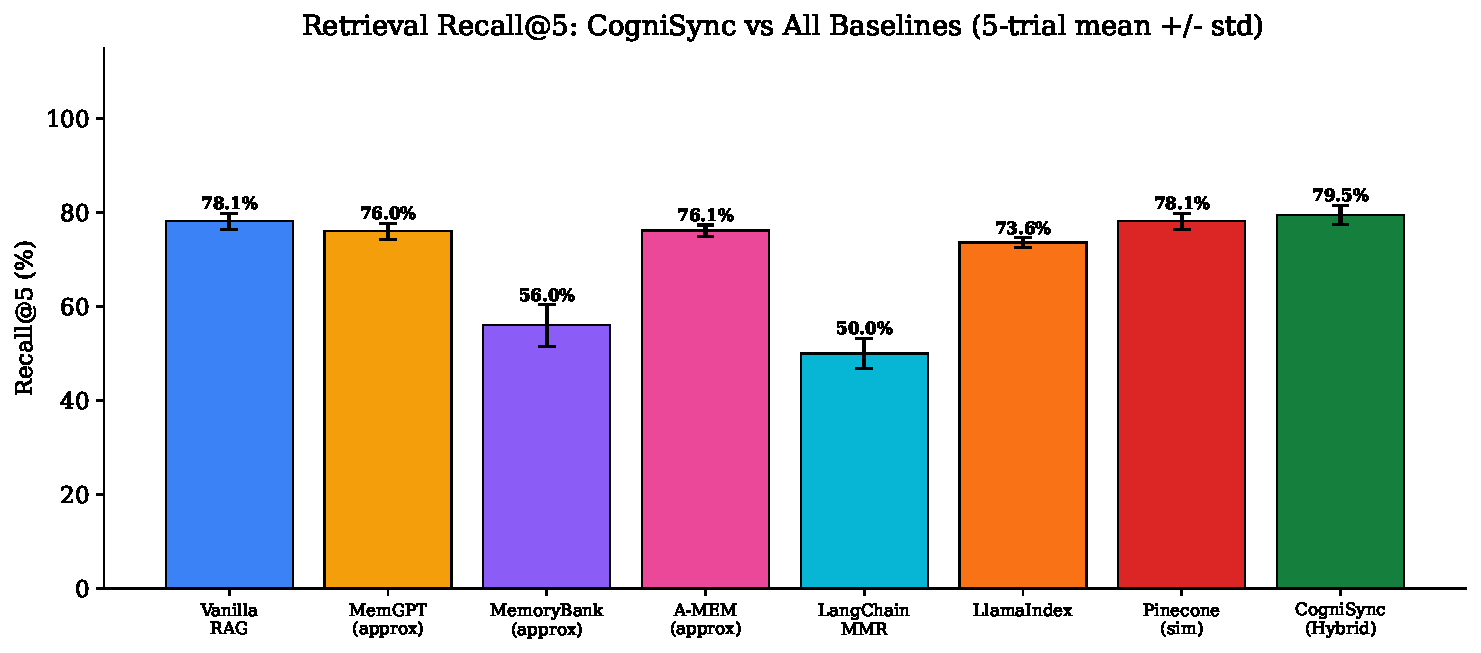
\includegraphics[width=0.96\textwidth]{figures/retrieval_recall_main.pdf}
\caption{Retrieval Recall@5 across all baselines (five-seed mean $\pm$ std). CogniSync attains the best overall Recall@5, but the visual also makes clear that the gain over a strong Vanilla RAG baseline is controlled rather than overwhelming.}
\label{fig:recall-main}
\end{figure*}

\subsection{Quality--Latency Tradeoff and Scalability}

CogniSync does not dominate dense-only retrieval on latency alone. Relative to Vanilla RAG, the hybrid stack adds 4.24\,ms mean latency because it executes both lexical and dense paths. The more relevant comparison is to a cloud-style managed-service setup: against Pinecone-sim, CogniSync is 7.8$\times$ faster (28.73\,ms versus 223.36\,ms) while delivering better retrieval quality.

Figure~\ref{fig:scale-main} shows that the local-first design remains practical as memory grows. Hybrid mean latency rises from 29.58\,ms at 2k documents to 51.67\,ms at 100k documents, while p99 latency remains below 75.54\,ms at the largest setting. Importantly, hybrid retrieval remains non-regressive relative to the paired dense-only baseline in the saved sweep: the mean R@5 gain is +0.00 points at 2k, +1.67 at 10k, +0.83 at 50k, and +0.83 at 100k. This is a useful systems result: the hybrid branch does not collapse as the memory footprint becomes large enough to stress local inference and indexing.

\begin{figure*}[t]
\centering
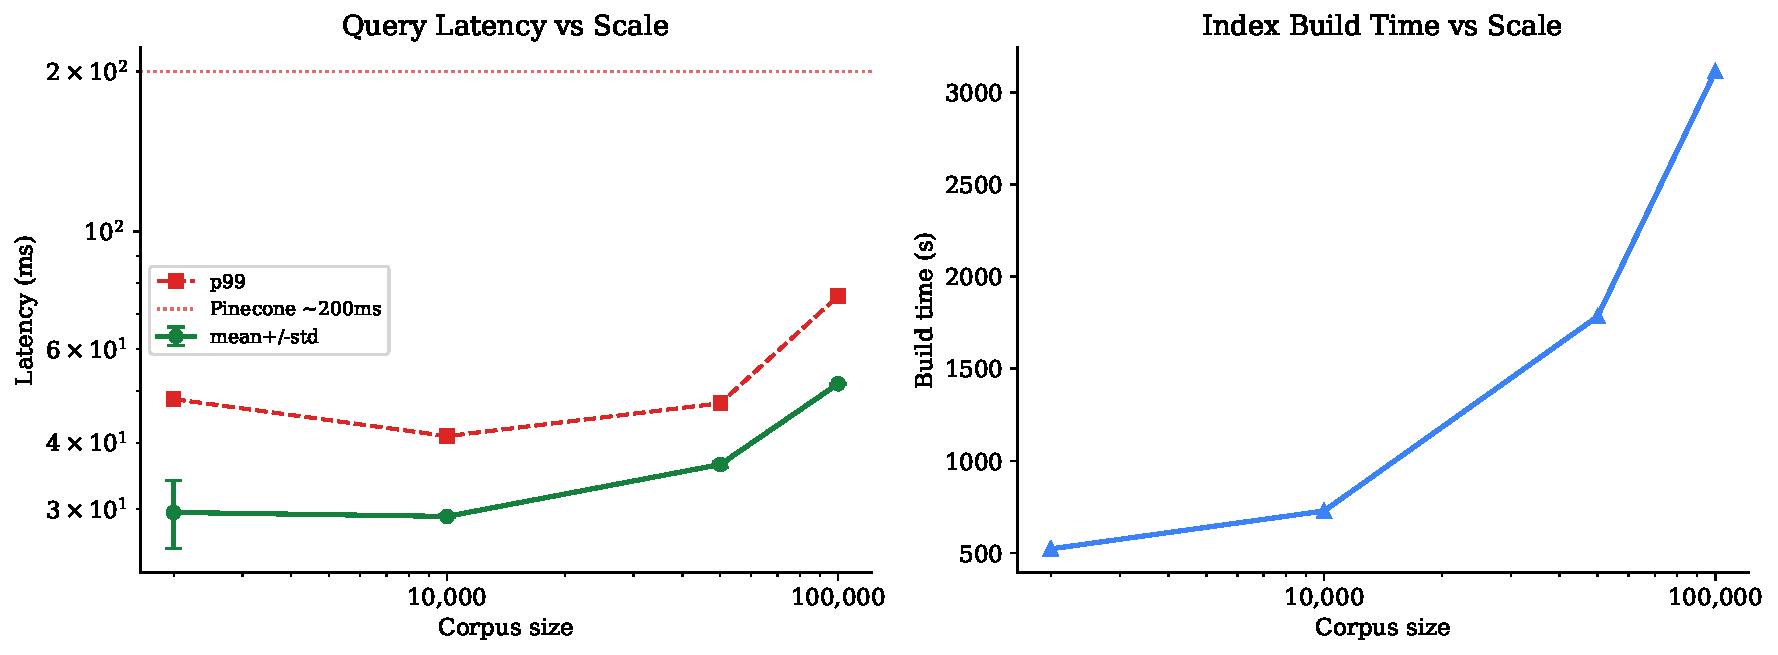
\includegraphics[width=0.96\textwidth]{figures/latency_scale_main.pdf}
\caption{Scalability results. Left: CogniSync mean latency (with std bars) and p99 latency remain well below the Pinecone-sim reference line as corpus size grows. Right: index build time increases with scale but remains practical for offline memory construction.}
\label{fig:scale-main}
\end{figure*}

\subsection{Security Hardening}

Because persistent memory can turn into a durable exfiltration channel, security must be evaluated alongside retrieval quality. Table~\ref{tab:security} reports the five-seed adversarial-memory evaluation. In the released benchmark, poisoning rate remained zero for all conditions, so the current results should be read as leakage mitigation rather than a complete poisoning-resilience study. Even under that conservative interpretation, the reductions are substantial: prompt injection leakage falls from 90.0\% to 0.0\%, tool spoofing from 100.0\% to 3.8\%, and data-exfiltration leakage from 100.0\% to 7.0\%.

\begin{table}[t]
    \caption{Leakage risk across five seeds. The current benchmark supports a strong leakage-mitigation claim, not yet a full poisoning-resilience claim.}
    \label{tab:security}
    \centering
    \small
    \begin{tabular}{@{}lrrr@{}}
        \toprule
        \textbf{Attack} & \textbf{Raw leak (\%)} & \textbf{Sanitized leak (\%)} & \textbf{Reduction (\%)} \\
        \midrule
        Prompt Injection  & 90.0  & 0.0 & 100.0 \\
        Tool Spoofing     & 100.0 & 3.8 & 96.2 \\
        Data Exfiltration & 100.0 & 7.0 & 93.0 \\
        \bottomrule
    \end{tabular}
\end{table}

This is one of the clearest empirical strengths of the current system. Persistent memory is valuable only if it can be trusted not to become a stable exfiltration channel. The sanitization layer is simple, but on the present benchmark it materially changes the system's risk profile.

\section{Discussion and Limitations}

The central takeaway from the empirical study is that local-first memory should be evaluated as a systems operating point. CogniSync does not win by producing a massive jump over a strong dense retriever. Instead, it wins by improving quality consistently, preserving locality, and remaining far faster than a cloud-style proxy while adding explicit safety hardening.

This matters because developer memory is a mixed workload. Some failures are semantic misses, but many are near misses involving exact values, identifiers, or policy text under heavy distractor pressure. A hybrid architecture is therefore valuable even when its average improvement looks small: the recovered cases are often the ones that matter most to real project correctness.

The present study also has important limitations. First, the released retrieval benchmark includes 50 workflow-memory queries spanning seven workflows. This is useful for a first mixed benchmark, but it is not broad enough to support sweeping claims about all agent-memory workloads. Second, the workflow-memory subset is already strong for Vanilla RAG, which limits the observable headroom for hybrid gains. Third, Pinecone-sim is a modeled proxy baseline rather than a live production deployment. Fourth, the current adversarial benchmark strongly supports leakage mitigation, but poisoning rate remains zero in the released setup. Finally, CogniSync is still primarily an append-and-retrieve system and does not yet solve memory invalidation or belief revision.

\section{Conclusion}

We presented CogniSync, a local-first persistent memory system for MCP-based agent workflows. CogniSync combines WAL-backed lexical retrieval, dense vector search, deterministic state fragmentation, and memory sanitization into a single deployable substrate for local agent cognition. On the released mixed benchmark, it achieves the best overall retrieval quality across eight systems and five seeds, statistically improving over Vanilla RAG while remaining much faster than a managed-service proxy. On the security side, the sanitization layer reduces leakage risk by 93.0--100.0\% across the three attack settings we evaluated. A separate scalability sweep shows that the local-first design remains usable through 100k documents without catastrophic latency growth.

These results do not justify a claim of retrieval SOTA in the abstract. They justify a different and, we believe, more practically important claim: persistent agent memory can be designed as a local quality--latency--safety tradeoff that fits real MCP deployments. In that sense, CogniSync is best understood not merely as a retriever, but as a systems substrate for durable and safer agent behavior.

\clearpage
\appendix

\section{Additional Experimental Details}

\subsection{Benchmark Composition}

The released benchmark contains 20 workflows and 160 workflow-evaluation queries in total, but the main retrieval experiment uses the first 50 workflow-memory queries together with 100 distractor queries per seed. This subset spans seven workflows and three domains. We make this choice explicit because it is the primary reason the current benchmark should be interpreted as a strong first systems evaluation rather than a fully saturated benchmark of all agent-memory regimes.

\subsection{Operational Cost Notes}

Targeted retrieval changes the economics of agent execution. For a 2,000-document workspace with an average of 350 tokens per document, injecting the full workspace would require roughly 700,000 input tokens per query. CogniSync instead injects only the top-5 retrieved chunks, reducing the prompt budget to roughly 1,750 tokens. This is a 99.75\% reduction in upper-bound prompt load and roughly a 400$\times$ reduction in per-query token cost under common API pricing assumptions.

The fragmentation pipeline also introduces limited overhead relative to the retrieval loop. On a 100\,MB compressed state, gzip compression completes in 6.07\,s and the subsequent deterministic slicing step completes in 25.69\,ms. In other words, fragmentation is not free, but it is small enough to be dominated by compression and sufficiently cheap to enable practical synchronization into transient environments.

\section{Additional Quantitative Results}

\begin{figure*}[t]
\centering
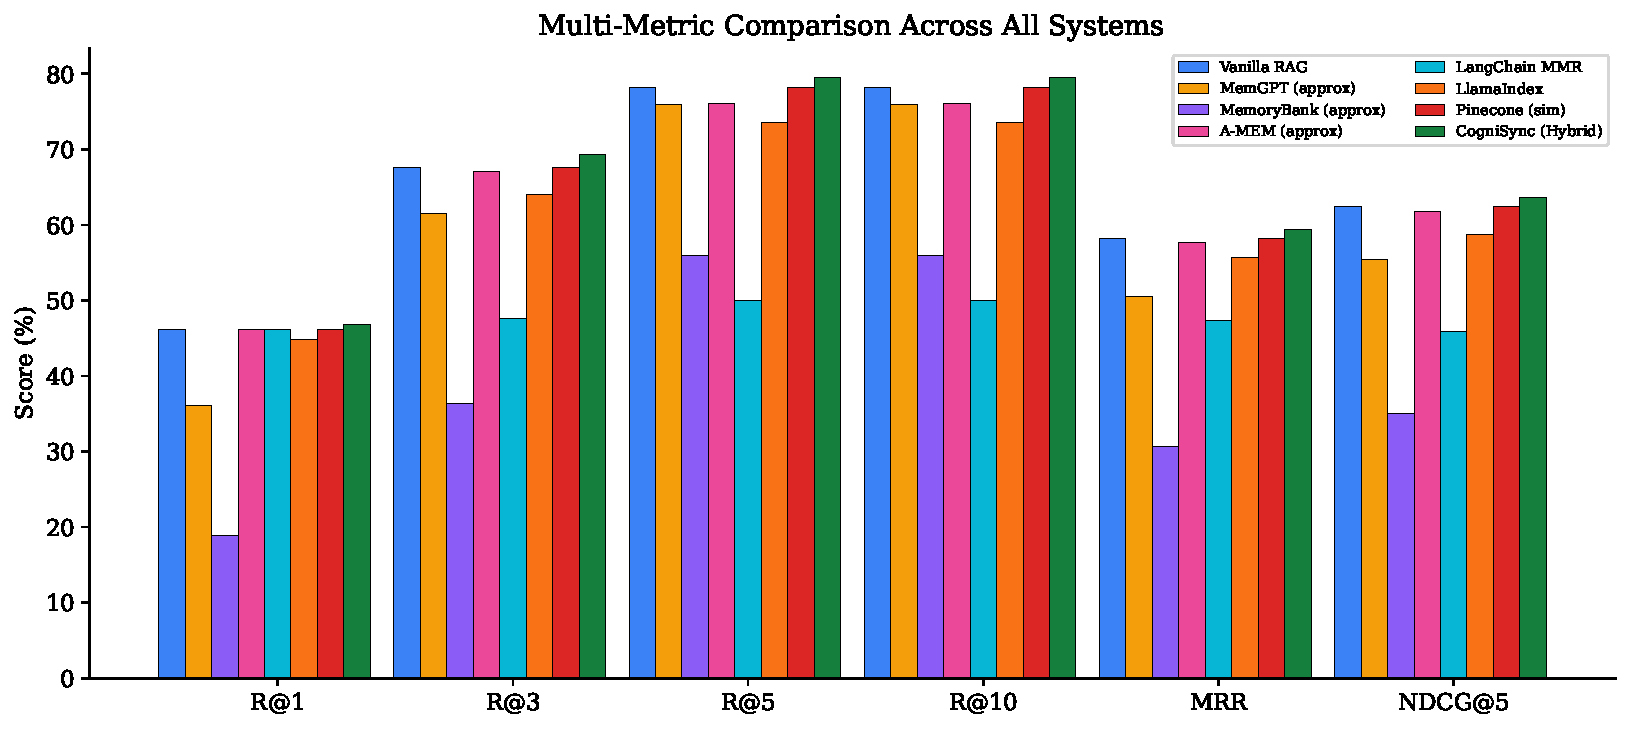
\includegraphics[width=0.96\textwidth]{figures/multi_metric_appendix.pdf}
\caption{Broader retrieval comparison across quality metrics. CogniSync leads on all reported retrieval measures, not only Recall@5.}
\label{fig:appendix-multi}
\end{figure*}

\begin{table}[t]
    \caption{Paired McNemar tests against CogniSync using pooled per-query hit vectors across seeds. ``CS-only'' counts queries solved only by CogniSync, while ``Base-only'' counts the converse.}
    \label{tab:stats}
    \centering
    \small
    \begin{tabular}{@{}lrrr@{}}
        \toprule
        \textbf{Baseline} & \textbf{$p$-value} & \textbf{CS-only} & \textbf{Base-only} \\
        \midrule
        Vanilla RAG         & 0.0063   & 11  & 1 \\
        MemGPT (approx)     & $5.0\times 10^{-6}$ & 28  & 2 \\
        MemoryBank (approx) & $2.6\times 10^{-39}$ & 177 & 1 \\
        A-MEM (approx)      & 0.00025  & 34  & 9 \\
        LangChain MMR       & $1.7\times 10^{-43}$ & 237 & 16 \\
        LlamaIndex          & $2.3\times 10^{-10}$ & 45  & 1 \\
        Pinecone (sim)      & 0.0063   & 11  & 1 \\
        \bottomrule
    \end{tabular}
\end{table}

\subsection{Agent-Oriented Task Evaluation}

\begin{figure*}[t]
\centering
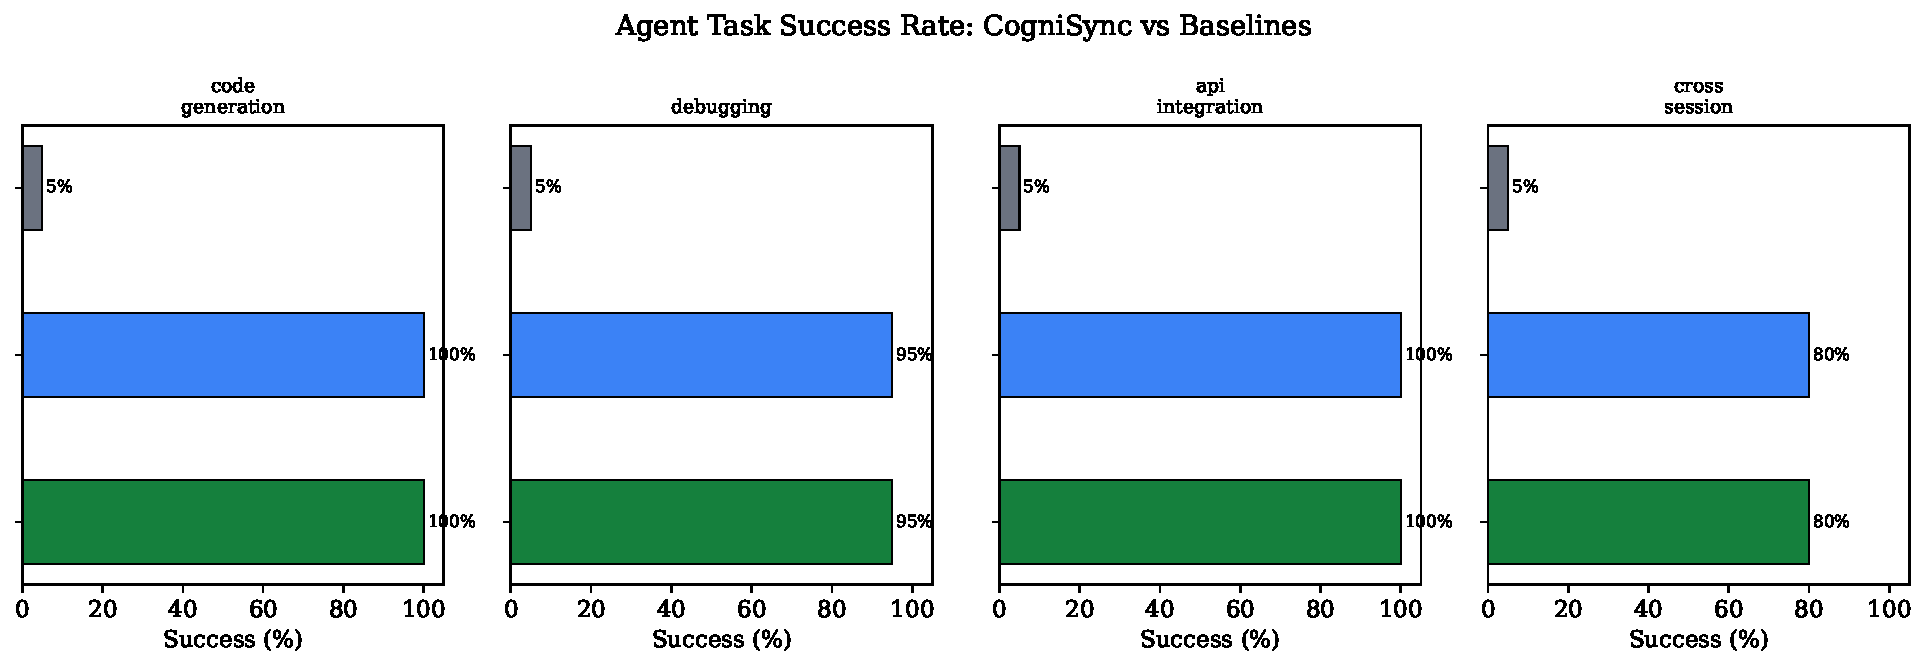
\includegraphics[width=0.96\textwidth]{figures/agent_tasks_appendix.pdf}
\caption{Agent-task success rates. CogniSync matches Vanilla RAG on success but not by large margins; the primary quantitative signal is that both memory-enabled systems dominate the zero-shot no-memory condition.}
\label{fig:appendix-agent}
\end{figure*}

\begin{table}[t]
    \caption{Agent-task evaluation summary. Success is largely saturated for the two memory-enabled systems; the most visible quality difference is a higher cross-session MRR for CogniSync.}
    \label{tab:agent}
    \centering
    \small
    \begin{tabular}{@{}lrrr@{}}
        \toprule
        \textbf{Task} & \textbf{CogniSync succ.} & \textbf{Vanilla succ.} & \textbf{CogniSync / Vanilla MRR} \\
        \midrule
        Code generation & 100.0 & 100.0 & 0.925 / 0.950 \\
        Debugging       & 95.0  & 95.0  & 0.787 / 0.783 \\
        API integration & 100.0 & 100.0 & 0.652 / 0.692 \\
        Cross session   & 80.0  & 80.0  & 0.739 / 0.698 \\
        \bottomrule
    \end{tabular}
\end{table}

\subsection{Security Visualization}

\begin{figure*}[t]
\centering
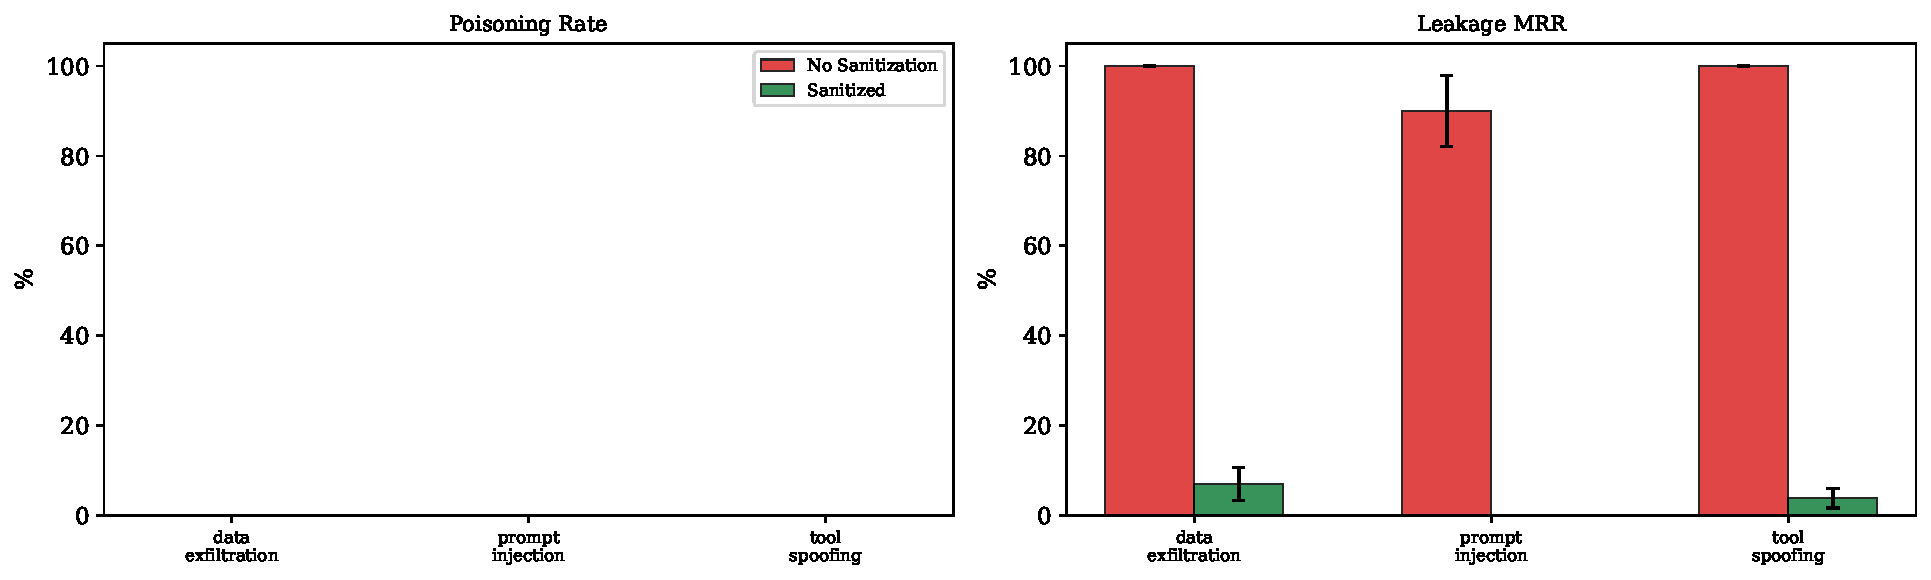
\includegraphics[width=0.96\textwidth]{figures/security_main.pdf}
\caption{Security evaluation visualization. The benchmark shows strong reductions in leakage risk after sanitization. The poisoning-rate panel is uninformative in the current release because poisoning remained zero across conditions, which is why the main paper reports these results as leakage mitigation rather than full poisoning resilience.}
\label{fig:appendix-security}
\end{figure*}

\section{Ablation Notes}

\begin{figure*}[t]
\centering
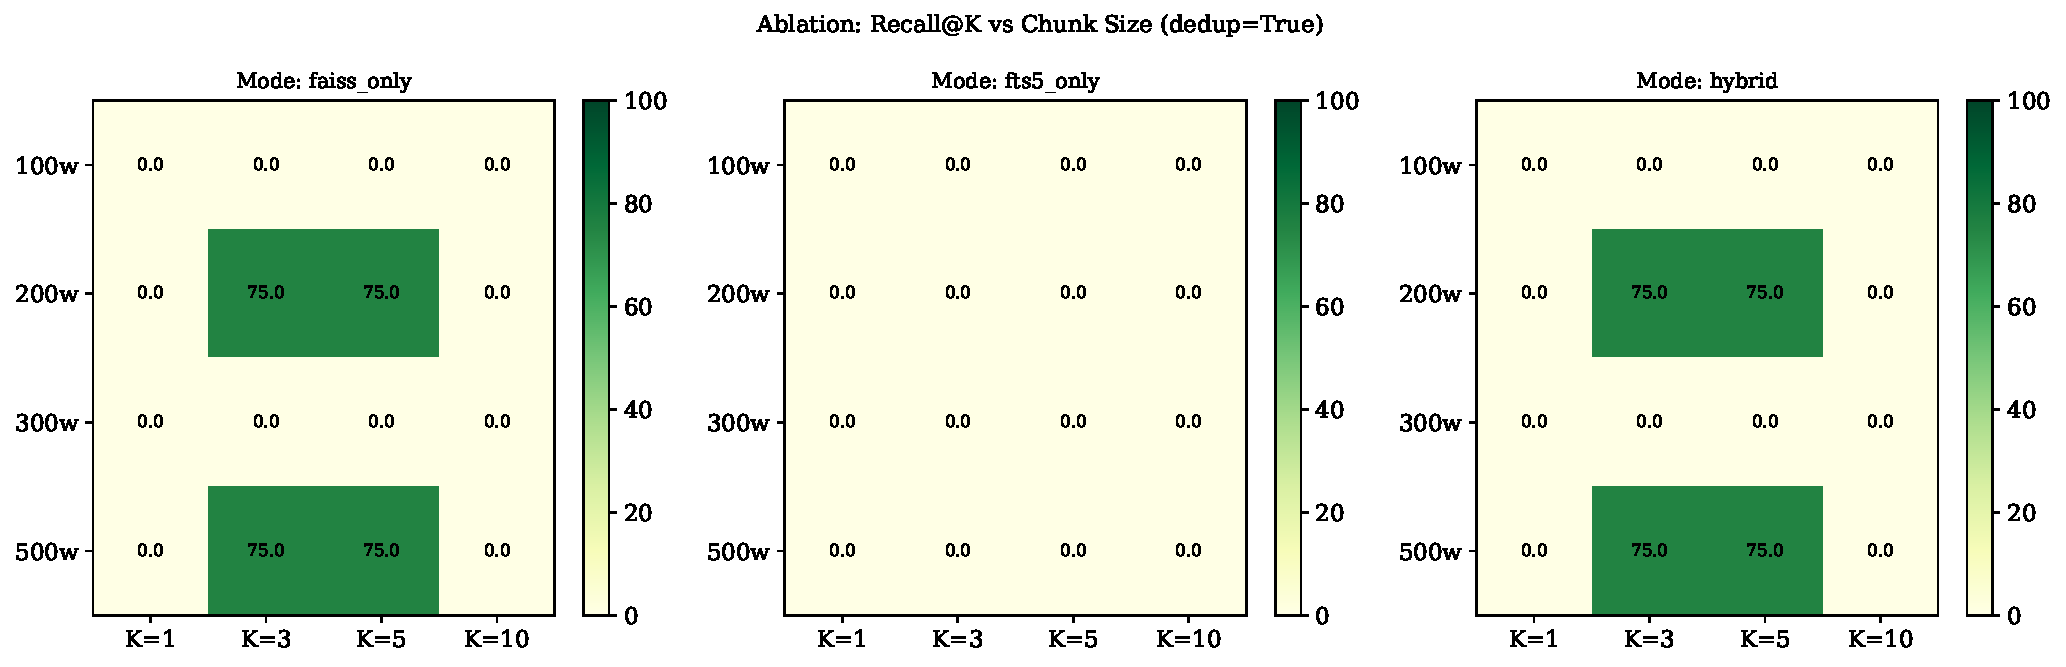
\includegraphics[width=0.96\textwidth]{figures/ablation_appendix.pdf}
\caption{Ablation heatmap from the released sweep. The current grid confirms that FTS5-only retrieval fails on this distractor-heavy setup, but it does not yet cleanly isolate where CogniSync's gains over dense-only retrieval come from. A sharper ablation benchmark remains future work.}
\label{fig:appendix-ablation}
\end{figure*}

The ablation study is informative but also reveals an evaluation gap. In the released sweep, the coarse configuration grid yields identical recall for the dense-only and hybrid settings at the tested chunk sizes and top-$K$ values, while FTS5-only retrieval collapses. This does not contradict the main result---the main benchmark still shows a statistically significant advantage for CogniSync over Vanilla RAG---but it does mean that the present ablation grid is too coarse to explain \emph{which} retrieval cases drive the observed gains. Future ablations should target conflict-heavy, identifier-heavy, and distractor-heavy regimes more directly.

\section{Qualitative Case Study}

We also recorded a simple two-session case study with a developer using Cursor connected to the CogniSync MCP server. In Session 1, the developer established a JWT design with 15-minute expiration and refresh-token rotation. In Session 2, opened days later in another service, the developer requested API gateway routing for a dashboard endpoint without restating the authentication policy. CogniSync retrieved the relevant JWT memory and the agent generated routing code consistent with the earlier design. In a matched control without CogniSync retrieval, the agent fell back to generic boilerplate and required manual reintroduction of the architectural constraints.

We do not treat this case study as primary quantitative evidence. Its value is explanatory: it illustrates the practical failure mode that motivates the system and shows how local persistent memory changes agent behavior when exact project decisions must survive session boundaries.

{\small\sloppy
\begin{thebibliography}{13}

\bibitem{lewis-rag}
P.~Lewis et al.
``Retrieval-Augmented Generation for Knowledge-Intensive NLP Tasks.''
In \emph{Advances in Neural Information Processing Systems 33}, 2020.

\bibitem{memorybank}
W.~Zhong et al.
``MemoryBank: Enhancing Large Language Models with Long-Term Memory.''
\emph{Proceedings of the AAAI Conference on Artificial Intelligence}, 38(17):19724--19731, 2024.

\bibitem{memgpt}
C.~Packer et al.
``MemGPT: Towards LLMs as Operating Systems.''
CoRR abs/2310.08560, 2023.

\bibitem{amem}
W.~Xu et al.
``A-MEM: Agentic Memory for LLM Agents.''
CoRR abs/2502.12110, 2025.

\bibitem{mcp-spec}
Model Context Protocol.
``Specification, version 2024-11-05.''
\url{https://modelcontextprotocol.io/specification/2024-11-05/index}

\bibitem{mcp-security}
S.~Gaire et al.
``Systematization of Knowledge: Security and Safety in the Model Context Protocol Ecosystem.''
CoRR abs/2512.08290, 2025.

\bibitem{mcpsecbench}
Y.~Yang, D.~Wu, and Y.~Chen.
``MCPSecBench: A Systematic Security Benchmark and Playground for Testing Model Context Protocols.''
CoRR abs/2508.13220, 2025.

\bibitem{beir}
N.~Thakur, N.~Reimers, A.~R\"uckl\'e, A.~Srivastava, and I.~Gurevych.
``BEIR: A Heterogeneous Benchmark for Zero-shot Evaluation of Information Retrieval Models.''
\emph{Proceedings of the Neural Information Processing Systems Track on Datasets and Benchmarks}, 1, 2021.

\bibitem{sqlite-wal}
SQLite Consortium.
``Write-Ahead Logging.''
\url{https://sqlite.org/wal.html}

\bibitem{faiss}
J.~Johnson, M.~Douze, and H.~J\'egou.
``Billion-scale similarity search with GPUs.''
\emph{IEEE Transactions on Big Data}, 7(3):535--547, 2021.

\bibitem{ann-benchmarks}
M.~Aum\"uller, E.~Bernhardsson, and A.~Faithfull.
``ANN-Benchmarks: A benchmarking tool for approximate nearest neighbor algorithms.''
\emph{Information Systems}, 87:101374, 2020.

\bibitem{serverless-state}
T.~Li, B.~Chandramouli, S.~Burckhardt, and S.~Madden.
``Serverless State Management Systems.''
In \emph{CIDR 2024}, 2024.

\bibitem{voiceagentrag}
J.~Qiu et al.
``VoiceAgentRAG: Solving the RAG Latency Bottleneck in Real-Time Voice Agents Using Dual-Agent Architectures.''
CoRR abs/2603.02206, 2026.

\end{thebibliography}
}

\end{document}
